\chapter{Electrosatics}
\section{The electric field}


\section{Example}
\begin{problem}
    Tìm điện trường tổng hợp của các điện tích trên đường trung trực $z$ của đoạn dây chiều dài $2L$, cách trung điểm $M$ của đoạn dây một khoảng $z$. Biết đoạn dây có mật độ điện tích dài là $\lambda$
\end{problem}

\textbf{Solution}

\begin{figure}[htbp]
    \centering
    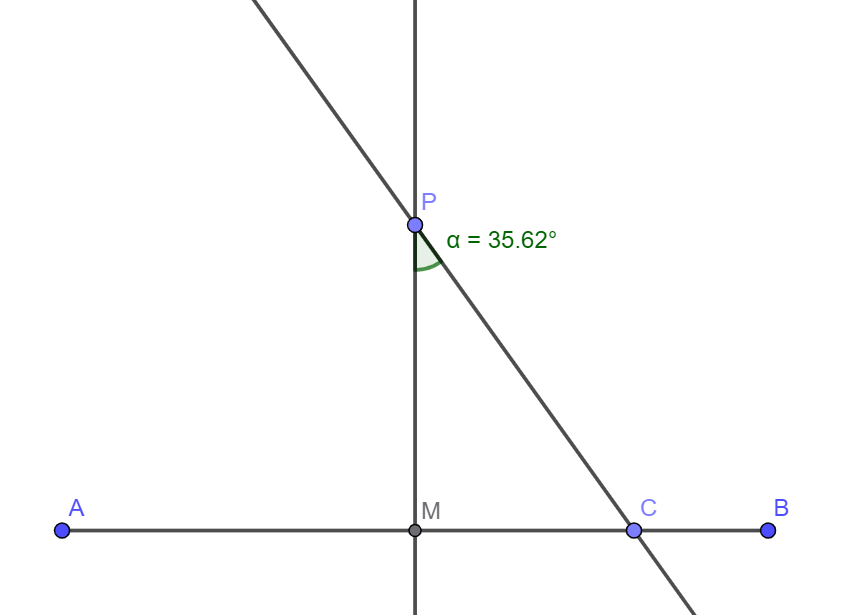
\includegraphics[width=0.6\textwidth]{p1_img.png}
    \label{fig:p1}
\end{figure}
Gọi $x$ là độ dài đoạn $MC$.
Theo nguyên lý chồng chập điện trường thì $E_{z} =  \Sigma dE_{z}$ mà \\
$E_{z} = E_{r} \cos \alpha$, lại có: $\cos \alpha = \frac{z}{r}$, $r = \sqrt{z^2+x^2}$\\ \\
\textbf{Nhận xét:} do tính đối xứng của đoạn dây qua đường trung trực $z$ nên. Điện trường trên đoạn dây bị triệt tiêu, lại có điện trường tác động lên các điện tích trên trục $z$ từ bên trái và bên phải đoạn dây đều bằng nhau nên.\\ \\
Áp dụng công thức tính điện trường ta được:

\begin{align*}
E_{z} &= 2\int_{0}^{L} 1\,dE_{z}\\
      &= 2\int_{0}^{L} 1\,d\frac{F_{z}}{Q_{z}}\\
      &= 2\int_{0}^{L} \frac{1}{r^2}\,dq\\
      &= 2\int_{0}^{L} \frac{\lambda z}{(z^2+x^2)^{3/2}}\,dx
\end{align*}

\section{Divergence and Curl of electrostatic fields}
\begin{enumerate}
    \item \textit{Electric Flux}\\
    Electric flux tiếng việt gọi là \textbf{điện thông} là đại lượng đo \textbf{mức độ điện  đi xuyên qua một mặt}.
Nếu tưởng tượng các đường sức điện như những sợi chỉ vô hình, thì Electric flux đếm xem có bao nhiêu sợi xuyên qua bề mặt đang xét và theo hướng nào.
\\ \\ 
Trong vật lý \textbf{điện thông} xuyên qua một bề mặt là vô hạn và liên tục, nó xuyên qua bề mặt từ mọi hướng nhưng do tính đối xứng, nên chỉ có hứng vuông gốc với mặt là được xét dẫn đến ta có công thức tính \textbf{điện thông} như sau:

\[
\Phi_E = \oint_{S} \mathbf{E}\cdot d\mathbf{a}
\]
\\
Ta xét bài toán tính điện thông xuyên qua mặt của vật bất kỳ. Khi này ta sử dụng phép phủ \textbf{Gauss}, tao bao phủ vật bởi quả cầu \textbf{Gauss}, do số lượng điện thông xuyên qua mọi mặt của vật đều xuyên qua các mặt của quả cầu \textbf{Gauss}. Dẫn đến ta chỉ cần tính điện thông trên mặt \textbf{Gauss} thì sẽ tính được điện thông trên các mặt của vật.
\\ \\
Khi này do mặt \textbf{Gauss} là mặt cầu và cũng là mặt $S$ trong công thức nên để tính được tiếp ta cần đổi sang hệ tọa độ cầu để tính.\\
Ta có công thức đổi biến sau:
\[
d\mathbf{a} = \hat{n} d\mathbf{x}d\mathbf{y} = \hat{n} \lVert J_\Phi \rVert d\mathbf{\phi}d\mathbf{\theta}
\]
Trong đó:
\[
\lVert J_\Phi \rVert = \lVert \vec{R}_\phi \times \vec{R}_\theta \rVert
\]
Vì ta đang xét trong tọa độ cầu nên:
\[
\vec{R}
=
\begin{bmatrix}
x\\
y\\
z
\end{bmatrix}
=
\begin{bmatrix}
r\sin\phi\cos\theta\\
r\sin\phi\sin\theta\\
r\cos\phi
\end{bmatrix}
\]
Suy ra:
\[
\vec{R}_{\phi}
=
\frac{\partial \vec{R}}{\partial \phi}
=
\begin{bmatrix}
r\cos\phi\cos\theta\\
r\cos\phi\sin\theta\\
- r\sin\phi
\end{bmatrix}
\qquad
\vec{R}_{\theta}
=
\frac{\partial \vec{R}}{\partial \theta}
=
\begin{bmatrix}
- r\sin\phi\sin\theta\\
r\sin\phi\cos\theta\\
0
\end{bmatrix}
\]
Từ đó ta tính được:
\begin{align*}
\lVert J_\Phi \rVert
&= \lVert \vec{R}_\phi \times \vec{R}_\theta \rVert \\[6pt]
&=
\left\|
\begin{bmatrix}
\hat{\phi} & \hat{\theta} & \hat{r}\\
r\cos\phi\cos\theta & r\cos\phi\sin\theta & -r\sin\phi\\
-r\sin\phi\sin\theta & r\sin\phi\cos\theta & 0
\end{bmatrix}
\right\| \\[8pt]
&=
\left\|
\hat{\phi} r^2 \sin^2\phi \cos\theta
+
\hat{\theta} r^2 \sin^2\phi \sin\theta
+
\hat{r} r^2 \sin\phi \cos\phi
\right\| \\[8pt]
&=
r^2 \sin\phi
\left\|
\begin{bmatrix}
\sin\phi\cos\theta\\
\sin\phi\sin\theta\\
\cos\phi
\end{bmatrix}
\right\| \\[8pt]
&=
r^2 \sin\phi
\sqrt{
\sin^2\phi\cos^2\theta
+
\sin^2\phi\sin^2\theta
+
\cos^2\phi
} \\[8pt]
&=
r^2 \sin\phi
\sqrt{
\sin^2\phi(\cos^2\theta+\sin^2\theta)
+
\cos^2\phi
} \\[8pt]
&=
r^2 \sin\phi
\sqrt{\sin^2\phi+\cos^2\phi} \\[8pt]
&=
r^2 \sin\phi
\end{align*}
Vậy suy ra:
\[
\|J_\Phi\|
=
r^2\sin\phi
\]
Dễ thấy \textbf{vector pháp tuyến} của mặt vi phân $d\mathbf{a}$ chính là vector bán kính $\mathbf{\hat{r}}$ quả cầu \textbf{Gauss}.Vậy công thức được viết lại thành:
\begin{align*}
\Phi_E &= \oint_{S} \frac{q \hat{r}}{r^2 4\pi \epsilon_{0}}\cdot \hat{r} \lVert J_\Phi \rVert d\mathbf{\phi}d\mathbf{\theta}\\[6pt]
       &= \oint_{S} \frac{q \hat{r}}{r^2 4\pi \epsilon_{0}}\cdot \hat{r} r^2\sin\phi d\mathbf{\phi}d\mathbf{\theta}\\[6pt]
       &= \frac{q}{4\pi \epsilon_{0}} \oint_{S} \sin\phi d\mathbf{\phi}d\mathbf{\theta}\\[6pt]
       &= \frac{q}{4\pi \epsilon_{0}} \iint_{(0;2\pi)\times(0;\pi)} \sin(\phi)\, d\theta d\phi \\[6pt]
       &= \frac{q}{4\pi \epsilon_{0}} \int_{0}^{2\pi}\, d\theta \int_{0}^{\pi} \sin(\phi)\, d\phi \\[6pt]
       &= \frac{q}{4\pi \epsilon_{0}} \int_{0}^{2\pi}\, 2d\theta \\[6pt]
       &= \frac{q}{4\pi \epsilon_{0}} 4\pi \\[6pt]
       &= \frac{q}{\epsilon_{0}}
\end{align*}
Bây giờ ta đã xác định được điện thông có được do một điện tích điểm gây ra bên trong một vật bất kỳ. Vậy nếu có nhiều điện tích điểm thì điện thông sẽ tính như nào ?\\[6pt]
Câu trả lời cũng không khó, ta hãy nhớ đến định luật chồng chập điện trường khi này:
\[
\mathbf{E}=\Sigma{\mathbf{E_{i}}}
\]
Từ đó ta tính được:
\[
\Phi_{\mathbf{E}} = \oint_{S} \mathbf{E}\ \cdot \, d\mathbf{a}=\oint_{S} \Sigma{\mathbf{E_{i}}} \cdot \, d\mathbf{a}=\Sigma \oint_{S} \mathbf{E_{i}}\ \cdot \, d\mathbf{a}=\Sigma \frac{q_{i}}{\epsilon_{0}}=\frac{Q_{enc}}{\epsilon_{0}}
\]
Với $Q_{enc}$ là tổng điện tích điểm có trong vật, mà tổng điện tích có trong vật có thể tính bằng công thức:
\[
Q_{enc} = \oint_{v} \rho\, d\tau
\]
Theo định lý \textbf{Greeen} ta lại có:
\[
\oint_{v} \nabla \cdot E \, d\tau = \oint_{s} E \cdot\, d\mathbf{a} 
\]
Suy ra:
\[
\oint_{v} \nabla \cdot E \, d\tau = \oint_{S} E \cdot\, d\mathbf{a} = \frac{Q_{enc}}{\epsilon_{0}}= \oint_{v} \frac{\rho}{\epsilon_0} \, d\tau
\]
Vậy:
\[
\boxed{\nabla \cdot E =\frac{\rho}{\epsilon_{0}}}
\]
Với $\rho$ gọi là mật độ điện tích khối.\\ \\
\textbf{Chú ý !!} Ta ký hiệu gốc cực và gốc phương vị này hơi khác so với định nghĩa tọa độ cầu ở trên, với \textbf{góc cực} là $\mathbf{\phi}$ còn \textbf{góc phương vị} là $\theta$.

\item \textit{The Divergence of E.}
Ta sẽ quay lại tính \textbf{Divergence} của $E$ khi mật độ điện tích khối phụ thuộc vào độ dài. Ta có,
\[
E(r) = \frac{1}{4 \pi \epsilon_{0}} \int_{\text{all space}} [\frac{\hat{\mathbf{r}}}{\mathbf{r}^2}\rho(r')] \, d\tau'
\]
Do $\mathbf{r} = r - r'$ và $\nabla \cdot (\frac{\mathbf{\hat{r}}}{\mathbf{r^2}}) = 4\pi\delta(\mathbf{r}^3)$ nên,
\begin{align*}
\nabla \cdot E &= \frac{1}{4 \pi \epsilon_{0}} \int_{\text{all space}} \nabla \cdot (\frac{\hat{\mathbf{r}}}{\mathbf{r}^2})\rho(r') \, d\tau'\\[6pt]
&=  \frac{1}{4 \pi \epsilon_{0}} \int_{\text{all space}} 4\pi \delta(r - r') \rho(r') \, d\tau'\\[6pt]
&= \frac{\rho(r)}{\epsilon_{0}}
\end{align*}
Đây chính là dạng vi phân của định lý Gauss, để khôi phục nó về dạng tích phân ta cũng làm tương tự phần trước,
\[
\int_{\mathbf{V}} \nabla \cdot E \, d \tau \,\, \overset{\text{Green}}{=} \,\, \oint_{\mathbf{S}} E \cdot \, da = \frac{1}{\epsilon_{0}}\int_{\mathbf{V}} \rho \, \tau = \frac{1}{\epsilon_{0}} Q_{enc}
\]



\item \textit{Applications of Gauss's Law.}
Ta tạm dừng phát triển lý thuyết để xem thử sức mạnh phi thường của định luật Gauss trong việc tính điện trường gây ra bởi mặt tích điện. Khi có đối xứng thích hợp, nó cung cấp phương pháp nhanh nhất và hiệu quả nhất để tính toán.
\begin{problem}
Tìm điện trường bên ngoài mặt cầu tích điện đều có bán kính là $r$ là tổng điện tích là $q$.
\end{problem}
\textbf{solution.}
Ta vẽ quả cầu có bán kính $r' > r$, giả sử điện trường bên ngoài mặt tồn tại khi này $E$ sẽ có hướng trùng với bán kính. Áp dụng định lý Gauss ta được,
\[
\oint_{S} E \cdot \, da =  \frac{Q_{enc}}{\epsilon_{0}}
\]
Lại có,
\[
Q_{enc} = q \qquad (\text{ đề bài cho tổng điện tích trên mặt $q$})
\]
do mặt cầu có tính đối xứng,
\begin{align*}
\oint_{S} E \cdot \, da &=  \oint_{S} \left| E \right|  \, da_{//} \\[6pt]
&= \left| E \right| \oint_{S}  \, da_{//} \\[6pt]
&= \left| E \right| 4\pi r'^{2}
\end{align*}
vậy,
\[
\left| E \right| 4\pi r'^{2} = \frac{q}{\epsilon{0}} \Leftrightarrow E = \frac{q}{4 \pi r'^{2} \epsilon_{0}}\hat{r'}
\]
\textbf{Nhận xét:} từ bài toán trên ta hình dung được những bước cơ bản để giải một bài toán tìm điện trường như sau.
\begin{enumerate}[label={}]
    \item \textbf{Bước 1:} vẽ mặt $Gauss$ thích hợp
    \item \textbf{Bước 2:} phân tích hướng của $E$ rồi áp dụng định lý Gauss
    \item \textbf{Bước 3:} sử dụng tính đối xứng để tính $E$
\end{enumerate}
Việc chọn mặt Gauss rất quan trọng vì nếu ta không chọn được mặt thì hợp thì $E$ sẽ không thể là hằng số vì không có tính đối xứng. Thông thường mặt Gauss được chọn sẽ là mặt có các tính đối xứng sau.
\begin{enumerate}[label={}]
\item{Sepherical symmtetry:} đối xứng cầu theo đó mặt được chọn để bao vật sẽ là mặt cầu.
\item 
\item{Cylindrical symmtetry:} đối xứng trụ theo đó mặt được chọn để bao vật sẽ là mặt trụ.
\item 
\item{Plane symmtetry:} đối xứng mặt theo đó mặt được chọn để bao vật sẽ là các mặt của hình hộp.
\end{enumerate}
Đặc biệt đối với \textbf{đối xứng trụ} và \textbf{đối xứng mặt} ta chỉ nên áp dụng khi đề bài cho khối trụ dài vô hạn hoặc mặt phẳng được mở rộng về mọi hướng. Điều này tương đương với dữ kiện "khối trụ dài" hay "mặt phẳng lớn" trong đề bài.

\begin{problem}
Cho một ống dài có mật độ điện tích tỉ lệ với khoảng cách đến trục: $\rho = ks$ với $k$ là hằng số. Tìm điện trường bên trong ống
\end{problem} 

\textbf{Solution.}
Ta vẽ khối trụ có chiều dài $l$ bán kính $s$, giả sử điện trường bên trong ống tồn tại khi này các đường sức điện sẽ hướng ra ngoài mặt trụ, áp dụng định luật Gauss ta được,
\[
\oint_{S} E \cdot \, da =  \frac{Q_{enc}}{\epsilon_{0}}
\]
Lại có,
\begin{align*}
Q_{enc} &= \oint_{V} \rho \cdot \, d \tau \\[6pt]
&= \iiint_V ks \, \, \, rdr d\phi dz \\[6pt]
&= \int_{0}^{l} \, dz \int_{0}^{2\pi} \, d\phi \int_{0}^{s} kr \, rdr \\[6pt]
&= 2\pi l \frac{ks^3}{3}
\end{align*}
do mặt trụ có tính đối xứng,
\begin{align*}
\oint_{S} E \cdot \, da &=  \oint_{S} \left| E \right|  \, da_{//} \\[6pt]
&= \left| E \right| \oint_{S}  \, da_{//} \\[6pt]
&= \left| E \right| 2\pi l s
\end{align*}
\textbf{Lưu ý:}vector pháp tuyến của hai mặt trên dưới khối trụ vuông góc với $E$ nên tích có hướng của nó với $E$ bằng không.
Vậy,
\[
\left| E \right| 2\pi l s = \frac{1}{\epsilon{0}} 2\pi l \frac{ks^3}{3} \Leftrightarrow E = \frac{k s^2}{3 \epsilon_{0}}\hat{s}
\]
\begin{problem}
Cho mặt phẳng dài vô hạn có mặt độ điện tích mặt là $\sigma$. Tìm điện trương sinh ra bởi mặt đó.
\end{problem}

\textbf{Solution.}
Ta vẽ hình hộp sao cho mặt phẳng chia đôi hộp, mặt trên của hộp có diện tích là $A$ mặt bên dưới cũng là $A$. Giả sử có điện trường được sinh ra bởi mặt, khi này $E$ sẽ hướng ra ngoài mặt sao cho chúng vuông góc với mặt. Áp dụng định lý Gauss ta được,
\[
\oint_{S} E \cdot \, da =  \frac{Q_{enc}}{\epsilon_{0}}
\]
Trong trường hợp này $Q_{enc} = \sigma A$ với $A$ là phần diện tích của nắp hộp. Sử dụng tính đối xứng ta được,
\[
\oint_{S} E \cdot \, da = \left| E \right| \oint_{S}  \, da_{//} = \left| E \right| 2A
\]
vậy,
\[
\left| E \right| 2A = \frac{1}{\epsilon_{0}}\sigma A \Leftrightarrow E = \frac{\sigma}{2\epsilon_{0}}\hat{n}
\]

\item \textit{The Curl of E.}
Rõ ràng về trực giác ta thấy rằng $E$ chỉ có div nên curl của $E$ sẽ bằng không. Nhưng ta sẽ không thừa nhận như vậy, ta sẽ chứng minh nó bằng cách khác.
\[
E = \frac{q}{4\pi\epsilon_{0}r^2}\hat{r}
\]
Ta lấy tích phân đường từ hai điểm $a$, $b$ bất kì,
\[
\int_{a}^{b} E \cdot \, dI
\]
Xét hệ tọa độ cầu,
\[
dI = dr + rd\theta + r\sin{\theta}d\phi 
\]
vậy
\begin{align*}
\Rightarrow \int_{a}^{b} E \cdot \, dI &= \int_{a}^{b} \frac{q}{4\pi\epsilon_{0}r^2} \, dr \\[6pt]
&= \frac{-q}{4\pi\epsilon_{0}r} \Big|_{a}^{b}\\[6pt]
&= \frac{q}{4\pi\epsilon_{0}}(\frac{1}{r_{a}} - \frac{1}{r_{b}})\\[6pt]
&= 0
\end{align*}
Kết quả trên là đúng vì $r_{a},r_{b}$ là bán kính nên chúng phải bằng nhau, đúng ra ta sẽ phải đổi cận khi đổi biến để tránh hiểu lầm nhưng do ta có thể viết gọn như trên nên bạn đọc có thể ngầm hiểu $a,b$ không nằm trên mặt cầu mà chính do phép đổi biến đã giúp ta thu được kết quả trên. Vì $a,b$ tùy ý nên,
\[
\oint E \cdot \, dI = 0
\]
Áp dụng định lý \textbf{Stokes} ta được,
\[
\oint E \cdot \, dI = \int_{S} (\nabla \times E) \cdot \, da = 0
\]
vậy,
\[
\boxed{\nabla \times E = 0} 
\]

\item \textit{Introduction to Potential.}

Điện trường $E$ không phải là một hàm bất kỳ; nó là một trường vectơ rất đặc biệt, cụ thể là một trường có xoáy bằng $0$ ở mọi nơi. Ví dụ, trường $E = y\hat{x}$ không thể là một điện trường vì không có bất kỳ hệ điện tích nào, bất kể độ lớn hay vị trí của chúng, có thể tạo ra một điện trường như vậy.

Trong phần này chúng ta sẽ khai thác tính chất đặc biệt trên của điện trường để biến bài toán tìm vectơ $E$ phức tạp thành một bài toán đơn giản hơn nhiều. Ở \textbf{Chương 1} ta đã biết rằng nếu $\nabla \times E = 0$ ở mọi nơi thì sẽ tồn tại một hàm thế $V$ sao cho $E$ là gradient âm của hàm đó. Trong phần này ta sẽ làm rõ điều đó.

Bởi vì $\nabla \times E = 0$ nên tích phân đường của $E$ trên một vòng kín sẽ bằng $0$ (theo định lý Stokes). Khi đó tích phân không còn phụ thuộc vào đường đi từ $a$ đến $b$, nên ta có thể định nghĩa một hàm mới:
\[
V(\mathbf{r}) \equiv -\int_{\mathbf{O}}^{\mathbf{r}} E \cdot dI .
\]

Ở đây $\mathbf{O}$ là điểm mốc chuẩn mà ta chọn trước để $V$ chỉ còn phụ thuộc vào $\mathbf{r}$. Hàm này được gọi là điện thế (electric potential).

Rõ ràng hiệu điện thế giữa hai điểm $a$ và $b$ sẽ là:
\begin{align*}
V(\mathbf{b}) - V(\mathbf{a})
&= \int_{\mathbf{O}}^{\mathbf{a}} E \cdot dI 
   - \int_{\mathbf{O}}^{\mathbf{b}} E \cdot dI \\
&= \int_{\mathbf{b}}^{\mathbf{O}} E \cdot dI 
   + \int_{\mathbf{O}}^{\mathbf{a}} E \cdot dI \\
&= -\int_{\mathbf{a}}^{\mathbf{b}} E \cdot dI .
\end{align*}

Mặt khác, theo định lý cơ bản của gradient:
\[
V(\mathbf{b}) - V(\mathbf{a}) 
= \int_{\mathbf{a}}^{\mathbf{b}} (\nabla V)\cdot dI .
\]

Vì vậy:
\[
\int_{\mathbf{a}}^{\mathbf{b}} (\nabla V)\cdot dI 
= -\int_{\mathbf{a}}^{\mathbf{b}} E \cdot dI .
\]

Điều này đúng với mọi $\mathbf{a},\mathbf{b}$ nên:
\[
E = -\nabla V.
\]
Phương trình trên chính là dạng vi phân của phương trình $V(\mathbf{r}) \equiv -\int_{\mathbf{O}}^{\mathbf{r}} E \cdot dI .$ Nó phát biểu rằng gradient của điện trường là một hàm thế vô hướng đúng như những gì ta muốn chứng minh.


Đừng để dấu trừ trong công thức làm bạn bối rối nó đơn giản chỉ là quy ước. Nhân tiện vai trò của việc tích phân độc lập với đường đi là cực kì quan trọng (tương đương với $\nabla \times E = 0$) vì nếu nó phụ thuộc vào đường đi thì định nghĩa của $V$ sẽ trở nên vô nghĩa.
\item \textit{Comments on Potential.}

\begin{enumerate}
\item \textbf{Tên Gọi:} Cái tên "thế" trong tên gọi thật sự rất dễ gây hiểu lầm vì nó làm ta liên tưởng ngay đến "thế năng", mặc dù chúng có liên quan với nhau khi ta đề cập đến chúng trong phần sau, nhưng về bản chất bạn cần phải hiểu rõ chúng là hai khái niệm hoàn toàn \textbf{khác nhau}.

\item \textbf{Lợi Thế:} Như ta đã biết việc tính được $V$ sẽ giúp ta dễ dàng suy ra được $E$ chỉ bằng cách lấy Gradient $E = -\nabla V$. Điều này thoạt nhìn có vẻ rất \textbf{ảo diệu} khi $V$ là đại lượng vô hướng chỉ gồm một thành phần trong khi $E$ là đại lượng vector ba thành phần. Nhưng nếu ta chú ý bởi vì điều kiện ban đầu $\nabla \times E = 0$ tương đương với,
\[
\frac{\partial{E_{x}}}{\partial{y}} = \frac{\partial{E_{y}}}{\partial{x}},
\qquad
\frac{\partial{E_{z}}}{\partial{y}} = \frac{\partial{E_{y}}}{\partial{z}},
\qquad
\frac{\partial{E_{x}}}{\partial{z}} = \frac{\partial{E_{z}}}{\partial{x}}
\]

\item \textbf{Điểm mốc:} Khi tính toán ta cũng nhận thấy được rằng việc chọn điểm mốc thật sự không ảnh hướng đến hiệu điện thế cũng như gradient vì việc thay đổi điểm mốc chính là cộng vào hàm điện thế ban đầu một hằng số $K$ hay $V(r') = K + V(r)$ điều này có thể dễ dàng suy ra từ định nghĩa hàm $V$. Do đó trong các bài toán về điện tích ta thường chọn điểm mốc ở \textbf{vô cực} nơi điện trường bằng 0 để tính toán. Nhưng cần lưu ý trong các bài toán về \textbf{mặt tích điện dài vô hạn} thì quy ước này sẽ trở nên vô dụng. Chẳng hạn cho mặt phẳng tích điện đều có điện trường,
\[
 E = \frac{\sigma}{2\epsilon_{0}}\hat{n}
\]
khi này,
\[
V(z) = -\int_{\infty}^{z} \frac{1}{2\epsilon_{0}} \, dz = -\frac{1}{2\epsilon_{0}}(z - \infty)
\]
Cách khắc phục là chọn mốc tham chiếu khác (trong bài toán này chính là gốc tọa độ). Lưu ý rằng các khó khăn kiểu như này ta chỉ gặp đối với các bài toán trong giáo trình, trong thực tế không có phân bố điện tích nào kéo dài vô tận, nên ta hoàn toàn có thể chọn \textbf{vô cùng} là mốc.
\item \textbf{Điện Thế Cũng Tuân Theo Nguyên Lý Chồng Chất:} Phát biểu đơn giản như sau: điện thế tại một điểm bất kỳ sẽ bằng tổng điện thế được gây ra bởi các điện tích riêng rẽ,
\[
V = V_{1} + V_{2} + V_{3} + ...
\]
\item \textbf{Đơn Vị:} Trong hệ SI điện thế có đơn vị là \textbf{Volt} hay Newton.Mét/Coulomb.
\end{enumerate}

\begin{problem}
Tìm điện thế bên trong và bên ngoài của mặt cầu bán kính là $R$. Có mật độ tích điện đều, chọn mốc ở vô cực.
\end{problem}

\textbf{Solution.} Từ định luật Gauss, ta có điện trường bên ngoài mặt cầu sẽ là:
\[
E = \frac{q}{4\pi\epsilon_{0}r^2} \hat{r}
\]
Vì điện tích chỉ tồn tại trên mặt cầu nên điện trường bên trong mặt sẽ bằng không. Với những điểm nằm ngoài mặt cầu ta bao chúng lại bằng một mặt cầu lớn hơn có $(\mathbf{r} > R)$.
\[
V(\mathbf{r}) = - \int_{\infty}^{\mathbf{r}} E \cdot \, dI = - \int_{\infty}^{r} \frac{q}{4\pi\epsilon_{0}r^2}\hat{r} \cdot \, dr\hat{r}
\]
Vì $dI = 
dr \hat{r}+
rd\theta\hat{\theta}+
r\sin(\phi)\hat{\phi}$ \,\,\,
vậy,
\[
V(\mathbf{r}) = \frac{q}{4\pi\epsilon_{0}r} \Big|_{\infty}^{\mathbf{r}} = \frac{q}{4\pi\epsilon_{0}\mathbf{r}}
\]
Với những điểm nàm trong mặt cầu ta sẽ tính như sau $(\mathbf{r}<R)$,
\[
V(\mathbf{r}) = - \int_{\infty}^{\mathbf{r}} E \cdot \, dI = - \int_{\infty}^{R} E \cdot \, dI - \int_{R}^{\mathbf{r}} E \cdot \, dI
\]
rõ ràng trong mặt cầu thì $E = 0$ nên,
\[
V(\mathbf{r}) = - \int_{\infty}^{\mathbf{r}} E \cdot \, dI = - \int_{\infty}^{R} \frac{q}{4\pi\epsilon_{0}r^2}\hat{r} \cdot \, dr\hat{r} - \int_{R}^{\mathbf{r}} 0 \cdot \, dr\hat{r} = \frac{q}{4\pi\epsilon_{0}R}
\]
\textbf{Nhận xét.} kết quả trên là hợp lý vì $E = -\nabla V = 0$ nên rõ ràng $V$ phải là trường hằng với những điểm nằm trong mặt cầu.
\item \textit{Poisson's Equation and Laplace's Equation}\\ \\
Trước đó ta đã chứng minh được công thức sau,
\[
E = -\nabla V 
\]
Câu hỏi đặt ra là, các phương trình cơ bản của $E$.
\[
\nabla \cdot E = \frac{\rho}{\epsilon_{0}} \qquad \text{và} \qquad \nabla \times E = 0
\]
sẽ được biểu diễn thế nào theo $V$. Ta có, $\nabla \cdot E = \nabla \cdot (-\nabla V) = -\nabla^2 V$. Nếu ta bỏ qua dấu trừ thì thật ra $E$ chính là \textbf{Laplacian} của $V$. Theo định luật Gauss,
\[
\nabla^2 V = -\frac{\rho}{\epsilon_{0}}
\]
Đây chính là phương trình \textbf{Poisson}. Trong trường hợp đặc biệt khi $\rho = 0$\, (không có điện tích) thì phương trình $Poisson$ sẽ trở thành phương trình $Laplacian$.
\[
\nabla^{2} V = 0
\]
Ta sẽ nghiên cứu cách giải phương trình này trong chương tiếp theo. Vậy còn Curl thì sao ? ta có,
\[
\nabla \times E = \nabla \times (-\nabla V) = 0
\]
điều này luôn đúng vì Curl của Gradient luôn bằng không, nó cho ta quan hệ quen thuộc. Có $\nabla \times E = 0$ thì tồn tại hàm vô hướng $V$ sao cho $E = -\nabla V$. Từ đây ta thấy rằng để xác định $V$ ta chỉ cần một phương trình là đủ đó chính là phương trình \textbf{Poisson}.
\item \textit{The Potential of a Localized Charge Distribution}\\ \\
Ở phần trước ta định nghĩa $E$ theo $V$, điều này đặc biệt hữu dụng vì thông thường nếu ta đi tính trực tiếp $E$ sẽ rất khó khăn, nhưng vì ta đã định nghĩa được $E$ thông qua $V$, dẫn đến ta chỉ cần tìm $V$ rồi lấy gradient thì cũng tính được $E$.
\\ \\
Theo phương trình \textbf{Poisson} ta được $\nabla^2 V = -\frac{\rho}{\epsilon_{0}}$ tức là nó cho ta biết giá trị của $\rho$ khi đã biết $V$ điều này trái với mong muốn của ta. Ta mong rằng khi có $\rho$ thì sẽ tính được $V$, do thế việc ta cần lầm là đảo ngược phương trình \textbf{Poisson}. Như thường lệ ta xét điện tích \textbf{ở gốc tọa độ},
\begin{figure}[htbp]
    \centering
    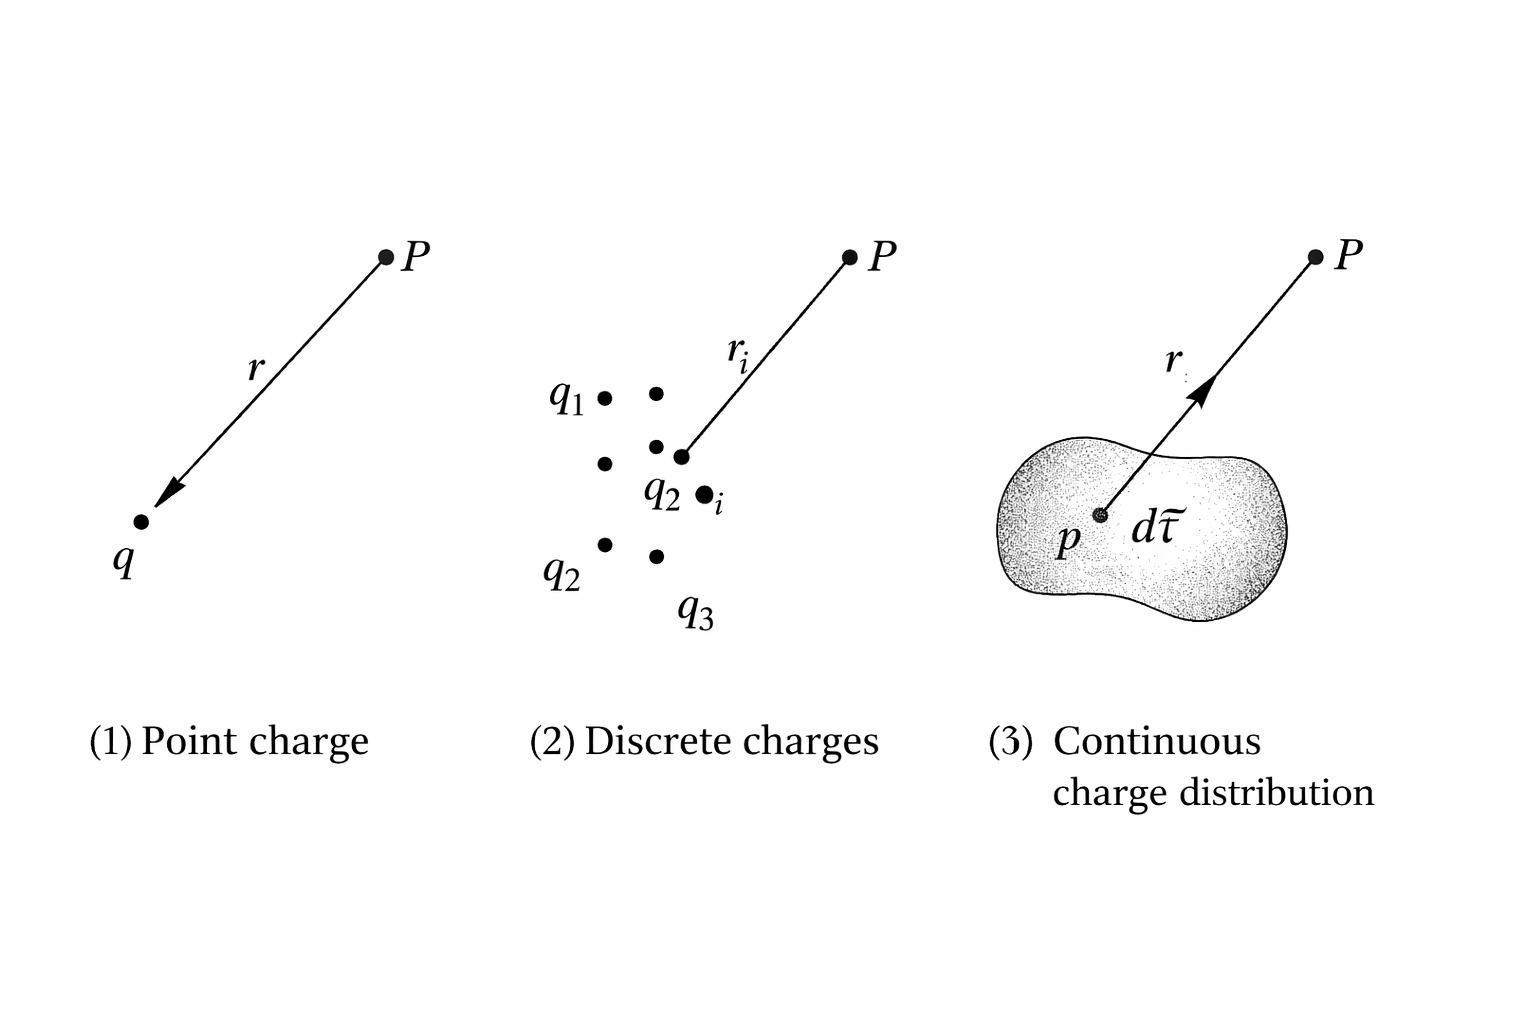
\includegraphics[width=0.6\textwidth]{phanbodientich.png}
    \label{fig:p1}
\end{figure}\\
Chọn gốc điện thế tại $\infty$ thì,
\[
V(r) = -\int_{\infty}^r E \cdot \, dI = -\int_{\infty}^r \frac{q}{4\pi\epsilon_{0}r'^2} \, dr' = \frac{1}{4\pi\epsilon_{0}}\frac{q}{r}
\]
Trong đó $r$ là khoảng cách từ gốc tọa độ đến điểm mà ta đang xét, nếu ta xét trong một hệ điện tích điểm thì,
\[
V(r) = \frac{1}{4\pi\epsilon{0}}\sum_{i=1}^{n} \frac{q_i}{r_i}
\] 
áp dụng lên một phân điện tích liên tục thì,
\[
V(r) = \frac{1}{4\pi\epsilon_{0}}\int \frac{1}{r} \, dq
\]
đặc biệt hóa trong trường hợp mật độ điện tích khối,
\[
\boxed{V(r) = \frac{1}{4\pi\epsilon_{0}}\int \frac{\rho(r')}{r} \, d\tau'}
\]
đây chính là nghiệm của phương trình \textbf{Poisson} nơi mà $V$  được tính khi đã biết $\rho$, điều thuận tiện khi tính kiểu này sẽ được thấy khi ta đem so sánh nó với công thức tính $E$ trước đó.
\[
E(r) = \frac{1}{4\pi\epsilon_{0}}\int \frac{\rho(r')}{r'^2}\hat{r'}\, d\tau '
\]
ta thấy ngay vector đơn vị $\hat{r'}$ phiền phức đã bị loại bỏ, dẫn đến việc tính toán trở nên rất đơn giản. Nhân tiện thì công thức tính $V$ đối với mật độ điện tích dài và mật độ điện tích mặt sẽ là,
\[
\frac{1}{4\pi\epsilon_{0}}\int \frac{\lambda(r')}{r} \, dl' \qquad \text{và} \qquad \frac{1}{4\pi\epsilon_{0}}\int \frac{\sigma(r')}{r} \, da'
\]
Lưu ý các công thức trên chỉ đúng khi $V(\infty) = 0$, nếu ngược lại tích phân sẽ phân kì.\\

\textbf{Example.} Tìm điện thế của một vỏ cầu tích điện đều có bán kính là $R$.\\
\begin{figure}[htbp]
    \centering
    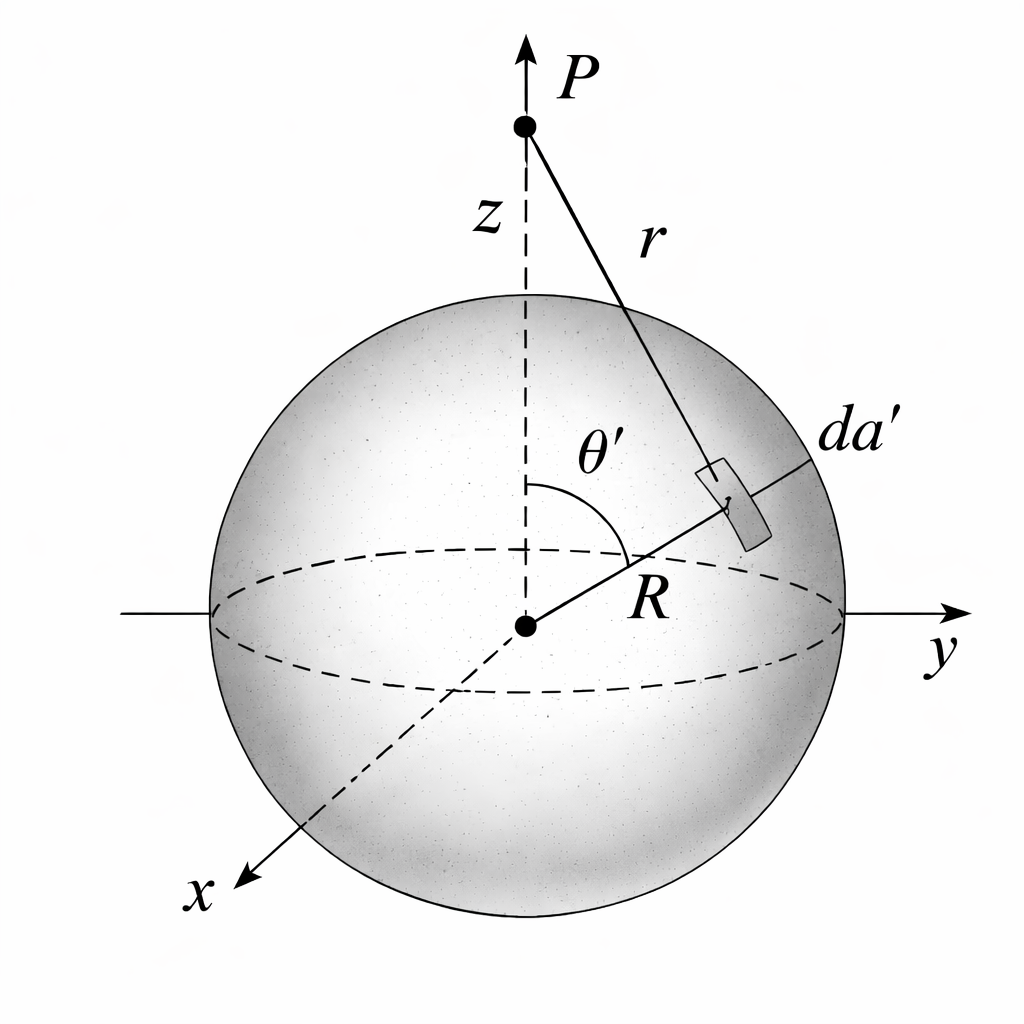
\includegraphics[width=0.6\textwidth]{dienthe1.png}
    \label{fig:p1}
\end{figure}
\textbf{Nhận xét} ta có những lưu ý vô cùng quan trọng trước khi giải bài,
\begin{enumerate}
\item Do hình cầu có đối xứng xuyên tâm nên việc đặt hệ trục tọa độ tại tâm của nó là tùy ý dẫn đến khi ta tính điện thế trên một hệ trục tọa độ nào đó thì nó cũng bằng điện thế tại các hệ trục tọa độ khác.

\item Ở phần lý thuyết điểm đặt điện tích của ta ở gốc tọa độ trong khi ở đây điểm đặt điện tích lại ở trên mặt cầu, dẫn đến $r'$ chính là khoảng cách từ điện tích trên mặt cầu tới điểm ta đang xét
\end{enumerate} 
\textbf{Solution.}Từ nhận xét ở trên ta chọn điểm nằm ngoài quả cầu và nằm trên trục $z$ như hình, khi đó điện thế của nó là,
\[
V(r) = \frac{1}{4\pi\epsilon_{0}}\int_{S} \frac{\sigma(r')}{r} \, da'
\]
do vỏ cầu tích điện đều nên $\sigma(r') = \sigma$ đổi hệ tọa cầu ta được,
\[
da' = \hat{n}dxdy = R^2\sin(\theta')d\phi'd\theta' \qquad \text{và} \qquad r'^2 = z^2 + R^2 -2zR\cos(\theta')
\]
dẫn đến,
\begin{align*}
V(r) &= \frac{\sigma}{4\pi\epsilon_{0}}\oint_{S} \frac{R^2\sin(\theta')d\phi'd\theta'}{\sqrt{z^2 + R^2 -2zR\cos(\theta')}} \\[6pt]
&= \frac{\sigma}{4\pi\epsilon_{0}}\iint_{(0;\pi) \times (0;2\pi)} \frac{R^2\sin(\theta')d\phi'd\theta'}{\sqrt{z^2 + R^2 -2zR\cos(\theta')}} \\[6pt]
&= \frac{\sigma}{4\pi\epsilon_{0}}\int_{0}^{\pi} \frac{R^2\sin(\theta')d\theta'}{\sqrt{z^2 + R^2 -2zR\cos(\theta')}} \int_{0}^{2\pi} \, d\phi'\\[6pt]
&= \frac{\sigma}{4\pi\epsilon_{0}}\int_{0}^{\pi} \frac{R^2\sin(\theta')d\theta'}{\sqrt{z^2 + R^2 -2zR\cos(\theta')}} 2\pi\\[6pt]
&= \frac{\sigma}{2\epsilon_{0}}\int_{-1}^{1} \frac{R^2dt}{\sqrt{z^2 + R^2 +2zRt}} \\[6pt]
&= \frac{\sigma}{2\epsilon_{0}} R^2 \frac{1}{Rz} \sqrt{z^2 + R^2 +2zRt} \Big|_{-1}^1 \\[6pt]
&= \frac{\sigma}{2\epsilon_{0}} \frac{R}{z} (\sqrt{z^2 + R^2 +2zR}-\sqrt{z^2 + R^2 -2zR}) \\[6pt]
&= \frac{\sigma R}{2z\epsilon_{0}} (\sqrt{(R+z)^2}-\sqrt{(R-z)^2})\\[6pt]
&= \frac{\sigma R^2}{z\epsilon_{0}} \qquad (\text{do điểm xét ở ngoài, $z > R$})
\end{align*}
tương tự, nếu điểm xét ở trong $z < R$ thì,
\[
V(r) = \frac{\sigma R}{\epsilon_{0}}
\]
kiểm tra lại ta thấy rằng
\[
E = -\nabla V = -\frac{\partial}{\partial z} \frac{\sigma R}{\epsilon_{0}}\hat{z} = 0 
\qquad \text{và} \qquad
E = -\nabla V = -\frac{\partial}{\partial z} \frac{\sigma R^2}{z\epsilon_{0}}\hat{z} = \frac{\sigma R^2}{z^2}\hat{z}
\]
Ứng với các điểm nằm trong và ngoài mặt cầu, thõa mãn các tính chất điện trường đã học.
\end{enumerate}
\section{Problems}

\begin{problem}
Một dây dẫn được uốn cong thành một cung tròn bán kình $R$, góc ở tâm là $\alpha$, mang điện tích phân bố đều với mật độ $\lambda \geq 0$. Tìm vector cường độ điện trường $\vec{E}$ tại $O$. Nhận xét trong trường hợp $\alpha$ là góc nhỏ. 
\end{problem}

\begin{figure}[htbp]
    \centering
    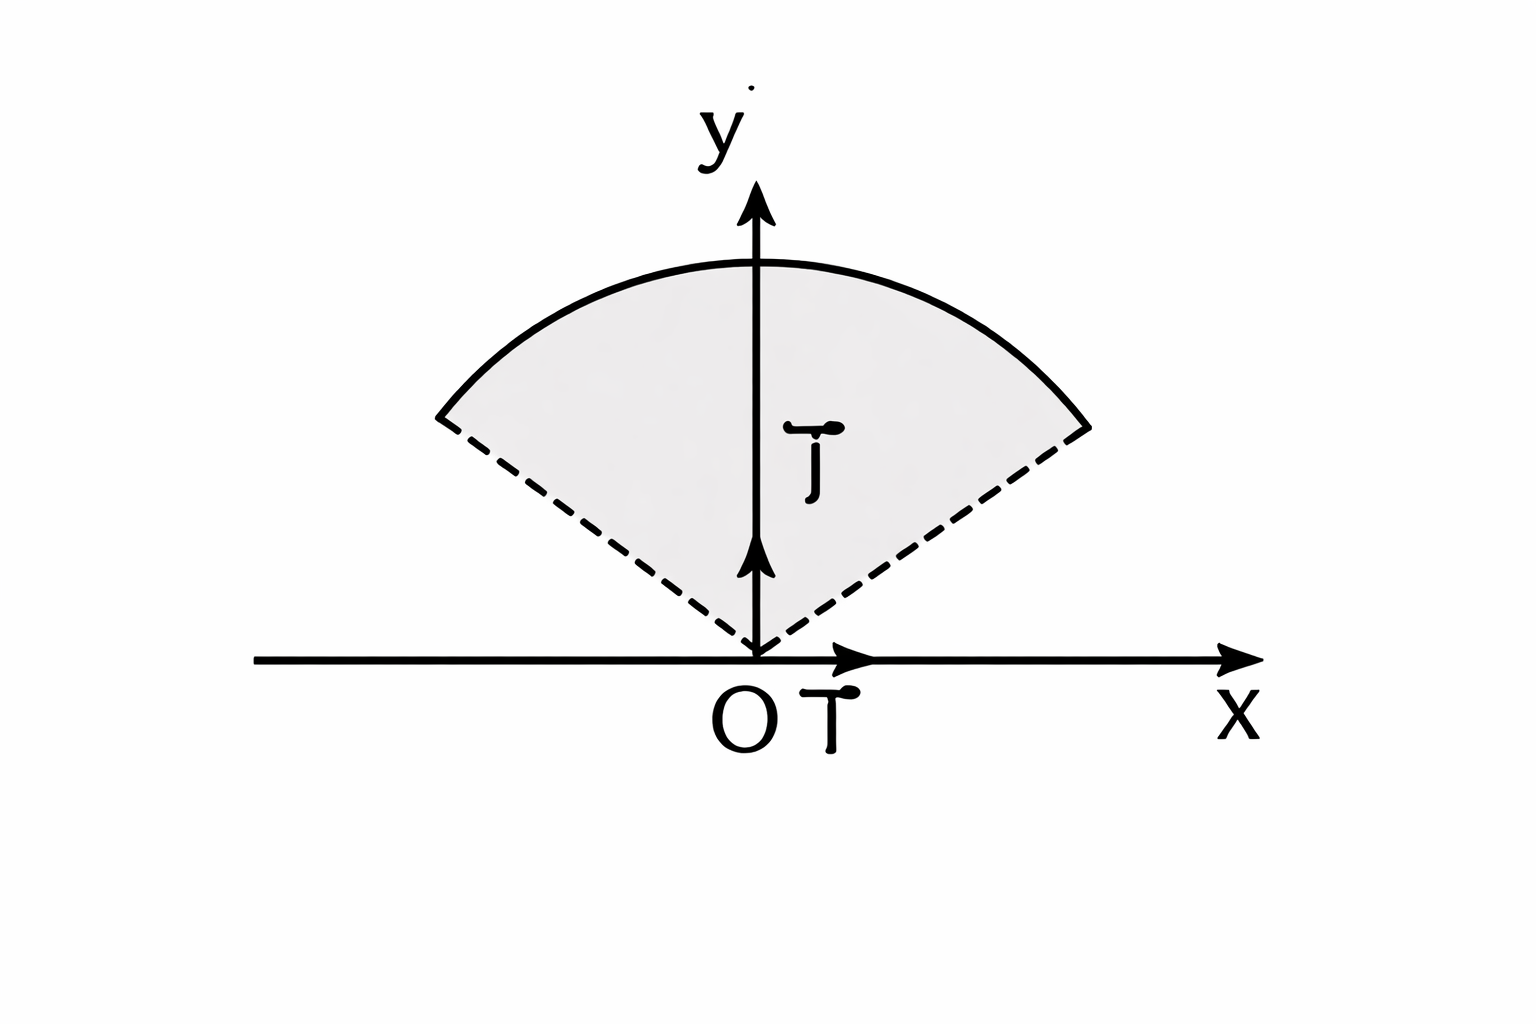
\includegraphics[width=0.6\textwidth]{problem2.6.png}
    \label{fig:p1}
\end{figure}
\textbf{Solution.} Chiếu $E$ lên phương $\vec{j}$, do tính đối xứng ta chỉ cần tính một nữa cung tròn rồi nhân hai ta có,
\[
E_{\perp} = \cos{\alpha'}E 
\]
Từ đó ta tính được,
\begin{align*}
E &= 2\int dE \\[6pt]
&= 2\int \cos{\alpha'}d E_{\perp}\\[6pt]
&= 2 \int \cos{\alpha'}\frac{kdq}{R^2}\\[6pt]
&= 2\int \cos{\alpha'}\frac{k\lambda dl'}{R^2}\\[6pt]
&= 2\int \cos{\alpha'}\frac{k\lambda Rd\alpha'}{R^2}\\[6pt]
&= 2\frac{k\lambda}{R}\int_{0}^{\frac{\alpha}{2}} \cos{\alpha'}\, d\alpha'\\[6pt]
&= 2\frac{k\lambda}{R} \sin{\alpha'} \Big|_0^{\frac{\alpha}{2}} \\[6pt]
&= 2\frac{k\lambda \sin{\frac{\alpha}{2}}}{R} 
\end{align*}
Vậy,
\[
\boxed{\vec{E} = -\frac{2k\lambda \sin{\frac{\alpha}{2}}}{R} \hat{R}}
\]
\begin{problem}
Một đĩa tròn bán kính $R$ được tích điện đều với mật độ điện tích mặt là $\sigma > 0$ và được đặt trong chân không. Xác định vector cường độ điện trường tại một điểm nằm trên trục đĩa và cáchtaam đĩa một khoảng $x$. Xét các trường hợp $x \gg R$ và $x \ll R$.
\end{problem}
\textbf{Solution.} Gọi $P$ là một điểm trên đĩa, ta xác định cường độ điện trường tại $M$ nằm trên trục đĩa,
\[
MP = \sqrt{r^2 + x^2}
\]
Chiếu vector cường độ điện trường lên trục thì,
\[
E = \cos{\alpha'}E_{\perp} = \frac{x}{\sqrt{r^2 + x^2}}E_{\perp}
\]
ta tính được,
\[
E = \int dE = \int \frac{x}{\sqrt{r^2 + x^2}} dE_{\perp} = k\sigma \oint_{S} \frac{x}{\sqrt{r^2 + x^2}} \frac{1}{x^2 + r^2} \, da
\]
đổi sang hệ tọa độ cực để tính tiếp,
\begin{align*}
    E &= k\sigma \oint_{S} \frac{x}{\sqrt{r^2 + x^2}} \frac{1}{x^2 + r^2} \, da\\[6pt]
     &= k\sigma \oint_{S} \frac{x}{(x^2 + r^2)^{\frac{3}{2}}} \, rdrd\phi\\[6pt]
     &= k\sigma \int_{0}^{2\pi} \, d\phi \int_{0}^{R} \frac{xr}{(x^2 + r^2)^{\frac{3}{2}}} \, dr\\[6pt]
     &= k\sigma \int_{0}^{2\pi} \, d\phi \int_{x^2}^{x^2 + R^2} \frac{x}{2t^{\frac{3}{2}}} \, dt\\[6pt]
     &= k\sigma \int_{0}^{2\pi} \, d\phi (\frac{-x}{\sqrt{t}})\Big|_{x^2}^{x^2+R^2} \, dt\\[6pt]
     &= k\sigma \int_{0}^{2\pi} \, d\phi (\frac{-x}{\sqrt{x^2}} + \frac{x}{\sqrt{x^2+R^2}}) \\[6pt]
     &= k\sigma 2\pi (\frac{x}{\sqrt{x^2+R^2}} -1) \\[6pt]
     &= \frac{\sigma}{2\epsilon_{0}} (\frac{x}{\sqrt{x^2+R^2}} -1)
\end{align*}
vậy,
\[
\boxed{\vec{E}= \frac{\sigma}{2\epsilon_{0}} (\frac{x}{\sqrt{x^2+R^2}} -1)\hat{r}}
\]
Nếu $x \gg R$ thì,
\[
E = \frac{\sigma}{2\epsilon_{0}}
\left(
\frac{x}{\sqrt{x^2+R^2}} - 1
\right)
=
\frac{\sigma}{2\epsilon_{0}}
\left(
\frac{1}{\sqrt{1+\frac{R^2}{x^2}}} - 1
\right)
\approx 0.
\]

Nếu $x \ll R$ thì,
\[
E = \frac{\sigma}{2\epsilon_{0}}
\left(
\frac{x}{\sqrt{x^2+R^2}} - 1
\right)
=
\frac{\sigma}{2\epsilon_{0}}
\left(
\frac{1}{\sqrt{1+\frac{R^2}{x^2}}} - 1
\right)
\approx -\frac{\sigma}{2\epsilon_{0}}.
\]
